%!TEX root = ../main.tex

\section{Emergent Interfaces}

\label{sec:emergent}

%%%%%%%%%%%%%%%%%%%%%%%%%%%%%%%%%%%%%%%%%%%%%%%%%%%%%%%%%%%%%%%%%%%%%%%%%

The problems discussed so far occur when features \textit{share} elements such as variables and methods, raising cross-feature dependencies. For instance, the common base code might declare a variable subsequently used by an optional feature (see \texttt{totalScore} and \texttt{status} in Figures~\ref{fig:arena-example} and~\ref{fig:gfilestatus-example}, respectively).

In this context, there are several paths to attack the problem with unclear cross-feature dependencies outlined in the previous section. The typical language-designer approach is to introduce additional modularity concepts into the programming language and make control-flow and data-flow explicit in interfaces, such as~\cite{shriram}. With \emph{emergent interfaces}, we pursue an alternative tool-based direction, which also works with existing languages and existing implementations and infers interfaces on demand.

%usar data flow na definicao. Em seguida, falar algo como: ``although we focus on data flow, we could use in control flow etc." Falar tambem que o Emergo so pegs dataflow.

To better explain what is an emergent interface, we first introduce maintenance points. \textit{Maintenance points are the code lines that the developer wants to change, for which she is interested in the cross-feature dependencies.} Also, we name \textit{impacted points the code lines we potentially impact if we change the maintenance points}. As any other code line, all these lines might be associated with feature expressions by using \texttt{\#ifdef} statements. Notice that one maintenance point---one code line---may impact many other code lines.

To define an emergent interface, let $MP$ be the set of maintenance points and $IP$ be the set of potentially impacted points. Also, let $FE(line)$ be a function that returns the feature expression associated with a given code line. This way, \textit{an emergent interface is a list of contracts in terms of ``$IP_i$ requires $MP_j$" emerging only if $FE(MP_j) \not\equiv FE(IP_i)$ and $FE(MP_j) \wedge FE(IP_i)$ is a valid feature expression}. Notice that for each contract of the list we have two elements: the maintenance point (the one that \textit{provides} data); and the impacted point (the one that \textit{requires} data). In other words, an emergent interface contains a list of contracts stating the code lines data dependent on the maintenance points. However, to emerge, each contract of the list must satisfy two constraints: the maintenance point and impacted point must have not equivalent feature expressions; and the conjunction of these expressions must be valid. The not equivalent constraint is necessary to compute cross-feature dependencies and the conjunction constraint prevents developers from assuming invalid dependencies.

Now, when developers are interested in dependencies from specific maintenance points, they can ask the tool that implements the technique to compute interfaces, pointing out feature dependencies. The interfaces emerge on demand, giving support for developers to maintain one feature without breaking others, since now they are aware of cross-feature dependencies. That is, the interfaces are inferred and shown in the IDE environment, instead of being written manually by developers.

To better illustrate how emergent interfaces work, we now refer to Figure~\ref{fig:eis}, which illustrates two maintenance tasks. When considering task~1, suppose there is something wrong with the initialization of variables \texttt{x}, \texttt{y}, and \texttt{k}. So, we should change them. Regarding task~2, we should change the \texttt{return} expressions of function \texttt{h}. For task~1, we select the following maintenance points (see the non-contiguous lines in dashed rectangles): lines $12$, $13$, $14$, and $27$ of \texttt{File F1}; afterwards, for task~2, we select lines $83$ and $85$ of \texttt{File F2}. 

%Figure~\ref{fig:eis} also makes explicit some feature constraints: features \texttt{A} and \texttt{B} are mutually exclusive; and feature \texttt{F} requires \texttt{!C}. Notice that this information might not be explicit in source code.

The emergent interfaces for tasks~1 and~2 contain six contracts and one contract, respectively. Each interface details, for each maintenance point, the potentially impacted statement, its line, its file, and the feature configuration in which the maintenance point impacts such a statement. We assume that the dots ``$\dots$" in Figure~\ref{fig:eis} do not contain any assignment to the variables we are interested during our maintenance tasks.

According to the emergent interface 1, if we change the statement \texttt{int x = 0} we impact the statements in lines $53$ and $87$, since they use the value of \texttt{x} and there is no path from the maintenance point to these lines where we assign a new value to \texttt{x}. Because we impact the statement \texttt{z = x + 9}, we transitively impact line $88$---\texttt{print(z)} statement---, since our maintenance in variable \texttt{x} contribute to define the value of \texttt{z} as well. This happens when we enable features \texttt{B}, \texttt{C}, and \texttt{D} (see column ``Feature Config."). When considering \texttt{y = g()} we impact line $87$ in products with \texttt{!A \&\& C \&\& D}. Due to the new assignment to \texttt{y} in feature \texttt{A}, this situation only occurs in case feature \texttt{A} is not enabled. Finally, if we change the assignment to variable \texttt{k} in line $14$ we impact lines $27$ in \texttt{File F1} and $33$ in \texttt{File F2}. To impact line $33$, the product must have feature \texttt{B} enabled and feature \texttt{E} not enabled. Notice that the maintenance point \texttt{k++} does not impact any line, including \texttt{i(k)}. According to the feature constraints at the bottom of Figure~\ref{fig:eis}, features \texttt{A} and \texttt{B} are mutually exclusive, so they do not impact each other. Therefore, we do not emerge any contract for this case---$FE($\texttt{i(k)}$) \wedge FE($\texttt{k++}$) = A \wedge B$ is not valid---preventing developers from assuming a non-existing dependency. Notice that constraints like this one might not be explicit in source code or even are unknown by developers.

According to the emergent interface 2, we impact only one point, i.e., line $87$ in \texttt{File F1}. The statement \texttt{return m + n} impacts the call to function \texttt{h} in products with \texttt{!F \&\& C \&\& D}. The statement \texttt{return m} does not impact such a call because if we enable feature \texttt{F}, we must disable feature \texttt{C} (see the constraint in Figure~\ref{fig:eis}).

Now, because developers are aware of cross-feature dependencies pointed by the emergent interface, they have better chances of not introducing errors to the code lines dependent on the maintenance points. In addition, developers do not need to reason about feature constraints hardly ever explicit in code; emergent interfaces already does it. Emergent interfaces also bring benefits to virtual separation and even for testing activities. We can improve comprehensibility (we hide the features not dependent of our task and focus on the ones we really care) and reduce effort by testing only the feature configurations pointed by our interfaces.

The tool we present next compute interfaces for a given set of maintenance points, helping developers to make code changes once they identify these points. Emergent interfaces do not contribute to finding the maintenance points in the first place, through.

%So, our interfaces play an important role on avoiding conflicts: by looking and analyzing the emergent interface, developers may have better chances of not introducing errors to the code lines dependent on the maintenance points. Thus, we provide treaties among features to resolve conflicts caused by cross-feature dependencies.

%To compute emergent interfaces, we use a feature-based slicing, which means we take feature constraints into account. We show the emergent interfaces for each task at the right-hand side of Figure~\ref{fig:eis}.

\begin{figure*}[ht]
\centering
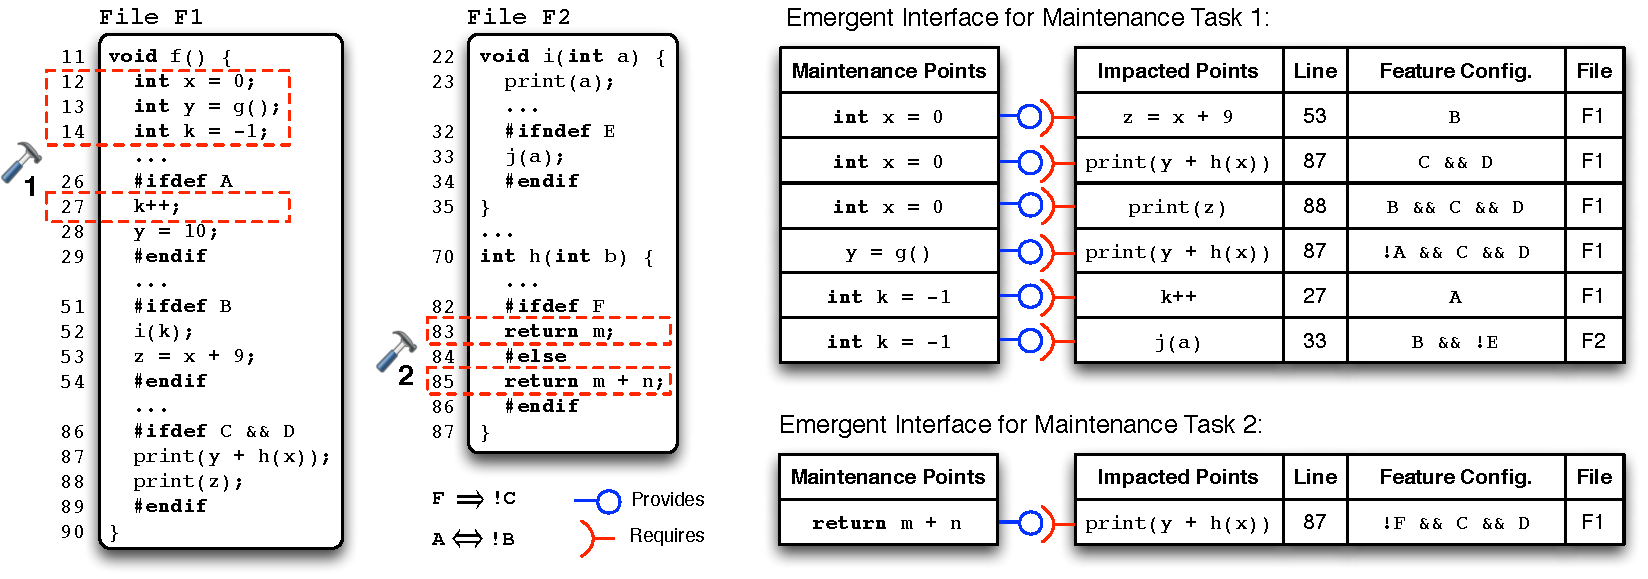
\includegraphics[width=0.92\textwidth]{images/EIs.pdf}
\caption{Examples of maintenance points and their respective emergent interfaces.}
\label{fig:eis}
\end{figure*}

%%%%%%%%%%%%%%%%%%%%%%%%%%%%%%%%%%%%%%%%%%%%%%%%%%%%%%%%%%%%%%%%%%%%%%%%%

%Now, we return to our scenarios from the previous section, using preprocessor-based implementations and views of virtual separation. 

%The problems discussed so far occur essentially because features \textit{share} values and behavior without clear interfaces. Whenever we have such sharing in the control flow or data flow, we say that there is a code level \textit{feature dependency} between the involved features~\cite{ribeiro-feature-dependencies-gpce11}. For instance, a mandatory feature might declare a variable subsequently used by optional features (see \texttt{totalScore} and \texttt{status} in Figures~\ref{fig:arena-example} and~\ref{fig:gfilestatus-example}, respectively).

%There are several paths to attack the problem with unclear cross-feature dependencies outlined in the previous section. The typical language-designer approach is to introduce additional modularity concepts into the programming language and make control-flow and data-flow explicit in interfaces, such as~\cite{shriram}. With \emph{emergent interfaces}, we pursue an alternative tool-based direction, which also works with existing languages and existing implementations and infers interfaces on demand.

%Emergent interfaces establish, on demand and according to a given code change task, interfaces to feature code. We use the following notion of interface: ``an interface is a way to resolve potential conflicts between the interacting parts of a design"~\cite{clark-design-rules-00}. Thus, we provide treaties among features to resolve conflicts caused by cross-feature dependencies. For example, an interface may state that a feature \textit{reads} a variable \textit{modified} by another.

%When developers are interested in dependencies from a specific code block, they can ask the tool that implements the technique to compute interfaces, pointing out feature dependencies. The interfaces emerge on demand, giving support for developers to maintain one feature without breaking others. That is, the interfaces are inferred and shown in the IDE environment, instead of being written manually by developers.

%To illustrate how emergent interfaces work, we return to our scenarios from the previous section, using preprocessor-based implementations and views of virtual separation. Consider \textit{Scenario 1}, where the developer is supposed to change how the total score is computed. The first step when using our approach consists of selecting the \emph{maintenance points}. A maintenance point is the point that the developer wants to change, for which she is interested in the interfaces to other features. In our case, the developer  manually selects the \texttt{totalScore} assignment as maintenance point (see the dashed rectangle in Figure~\ref{fig:arena-ei}) and then our tool analyzes the code to capture dependencies between the feature she is maintaining and the others. Finally, the interface emerges as shown in Figure~\ref{fig:arena-ei} (right-hand side).

%\begin{figure}[htp]
%\centering
%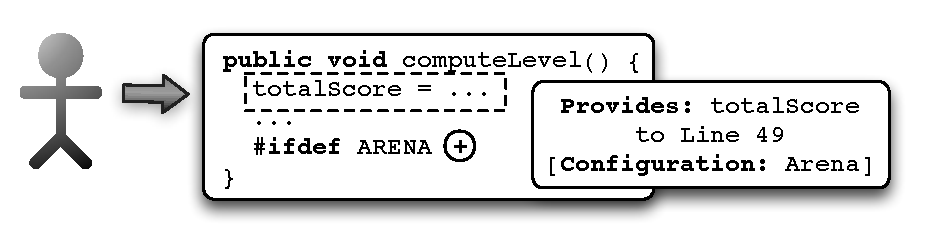
\includegraphics[width=0.45\textwidth]{images/Arena-EI.pdf}
%\caption{Emergent interface for Scenario 1.}
%\label{fig:arena-ei}
%\end{figure}

%The emerged interface states that the code change task may impact the behavior of products containing the \textit{ARENA} feature. So, the common code base provides \texttt{totalScore} current's value whereas \textit{ARENA} requires it. The developer is now aware of the dependency. When investigating it, she is likely to discover that she also needs to modify \textit{ARENA} code to avoid introducing an error.

%The tool we present next always compute interfaces for a given set of maintenance points, helping developers to make code changes once they identify these points. Emergent interfaces do not contribute to finding the maintenance points in the first place, through.

%Notice we do \textit{not} provide any support to find the maintenance points. This task is up to the developer according to her knowledge about the source code. After finding these points, she takes them as input to our approach. Then, we provide information about the potential features she might impact.

%This way, EIs focus on the features we indeed might impact, avoiding developers from the task of analyzing unnecessary features, being important to decrease \textit{Effort}. For instance, consider \textit{Scenario 2} (Section~\ref{sec:breaks}) in which we use the \texttt{status} variable in two optional features. Here, our interface ignores the \textit{SLINK} feature, since it does not use the \texttt{status} variable. Now, the navigation throughout the code is easier.

\subsection{Implementation: Emergo}

We implemented the concept of emergent interfaces in an Eclipse-based tool named Emergo. Emergo computes emergent interfaces based on feature dependencies between methods or within a single method, by using \textit{interprocedural} or \textit{intraprocedural} feature-sensitive data-flow analysis~\cite{brabrand-dfa4spl-aosd12, bodden-ifds4spl-pldi13}. This means we can take only valid feature combinations into account, preventing developers from reasoning about feature constraints and even from assuming invalid dependencies in case of mutually exclusive features (which may cause potential errors). Again, developers might assume that changing the \texttt{k++} assignment in feature \textit{A}---in Figure~\ref{fig:eis}---may lead to problems in feature \textit{B} (see the \texttt{i(k)} statement). Since the involved features are mutually exclusive, Emergo would not emerge any interface, which means that code change tasks in the former feature do not impact the latter, and vice-versa.

%\begin{figure}[htp]
%\centering
%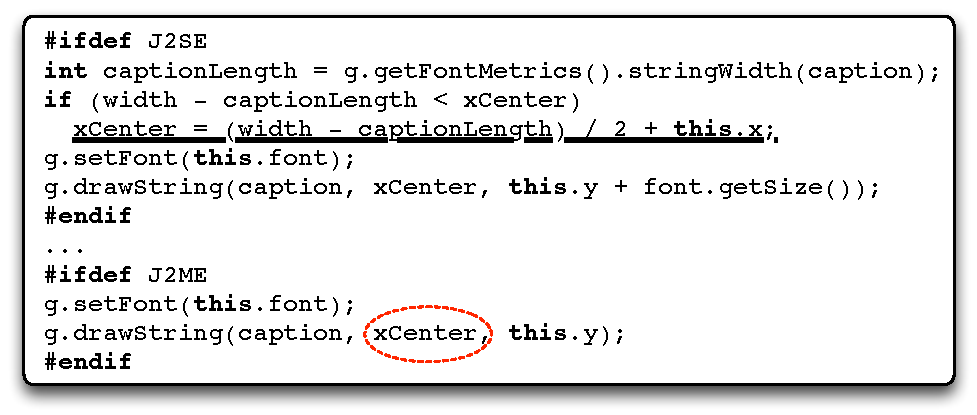
\includegraphics[width=0.5\textwidth]{images/Alternative.pdf}
%\caption{No dependency: mutually exclusive features.}
%\label{fig:emergo-alternative}
%\end{figure}

To illustrate Emergo in action, we return to our scenarios from the previous section. Consider \textit{Scenario 1}, where the developer is supposed to change how the total score is computed. The first step when using our approach consists of selecting the \emph{maintenance points}. In our case, the developer manually selects the \texttt{totalScore} assignment as maintenance point. Then, she would rely on Emergo to analyze the code to capture dependencies between the feature she is maintaining and the others. Finally, the interface emerges stating that the code change task may impact the behavior of products containing the \textit{ARENA} feature. So, the common code base provides \texttt{totalScore} current's value whereas \textit{ARENA} requires it. The developer is now aware of the dependency. When investigating it, she is likely to discover that she also needs to modify \textit{ARENA} code to avoid introducing an error.

Figure~\ref{fig:emergo} illustrates a screen shot of Emergo. After the developer found and selected the maintenance point in Line~1277 (the \texttt{totalScore} assignment), Emergo shows emergent interfaces using a table view and a graph view. To better understand the results pointed by Emergo, we now focus on the table. The ``Description" column illustrates the maintenance points. Since there is no \texttt{\#ifdef} statement encompassing the maintenance point, we associate it with the \textit{mandatory} feature. We show the potentially impacted configuration in the ``Feature" column, here with the \textit{ARENA} feature. The table view also shows the exact (impacted) lines of code that contain uses of \texttt{totalScore} as well as their respective files (see the ``Resource" column). In summary, we read the first line of the table as follows: if she changes the \texttt{totalScore} assignment belonging to the mandatory feature, she can potentially impact products with the \textit{ARENA} feature in line 177 of the \texttt{NetworkFacade} class.

Initially, Emergo shows all dependencies in both views. This way, depending on the project, it points lots of dependencies, which might be difficult to read and understand them. Thus, to focus on a particular one, she can click on the corresponding table line and Emergo automatically removes unrelated dependencies of the graph. This means we only show the path associated with the dependency of that table line. According to Figure~\ref{fig:emergo}, she selected the first line of the table. So, the graph now has only the path from the maintenance point to line 177 of the \texttt{NetworkFacade} class. 

Also, developers can reach the impacted feature code in the IDE editor by clicking either on table lines or on the graph nodes. For example, if she clicks on the node ``\texttt{score = (s < 0) ? 0 : s;}" of the graph, she reaches the code that checks the invariant that all scores are positive. Now, she is aware of the dependency. So, to accomplish the task of allowing negative scores she knows she also needs to remove the check.

\begin{figure*}[ht]
\centering
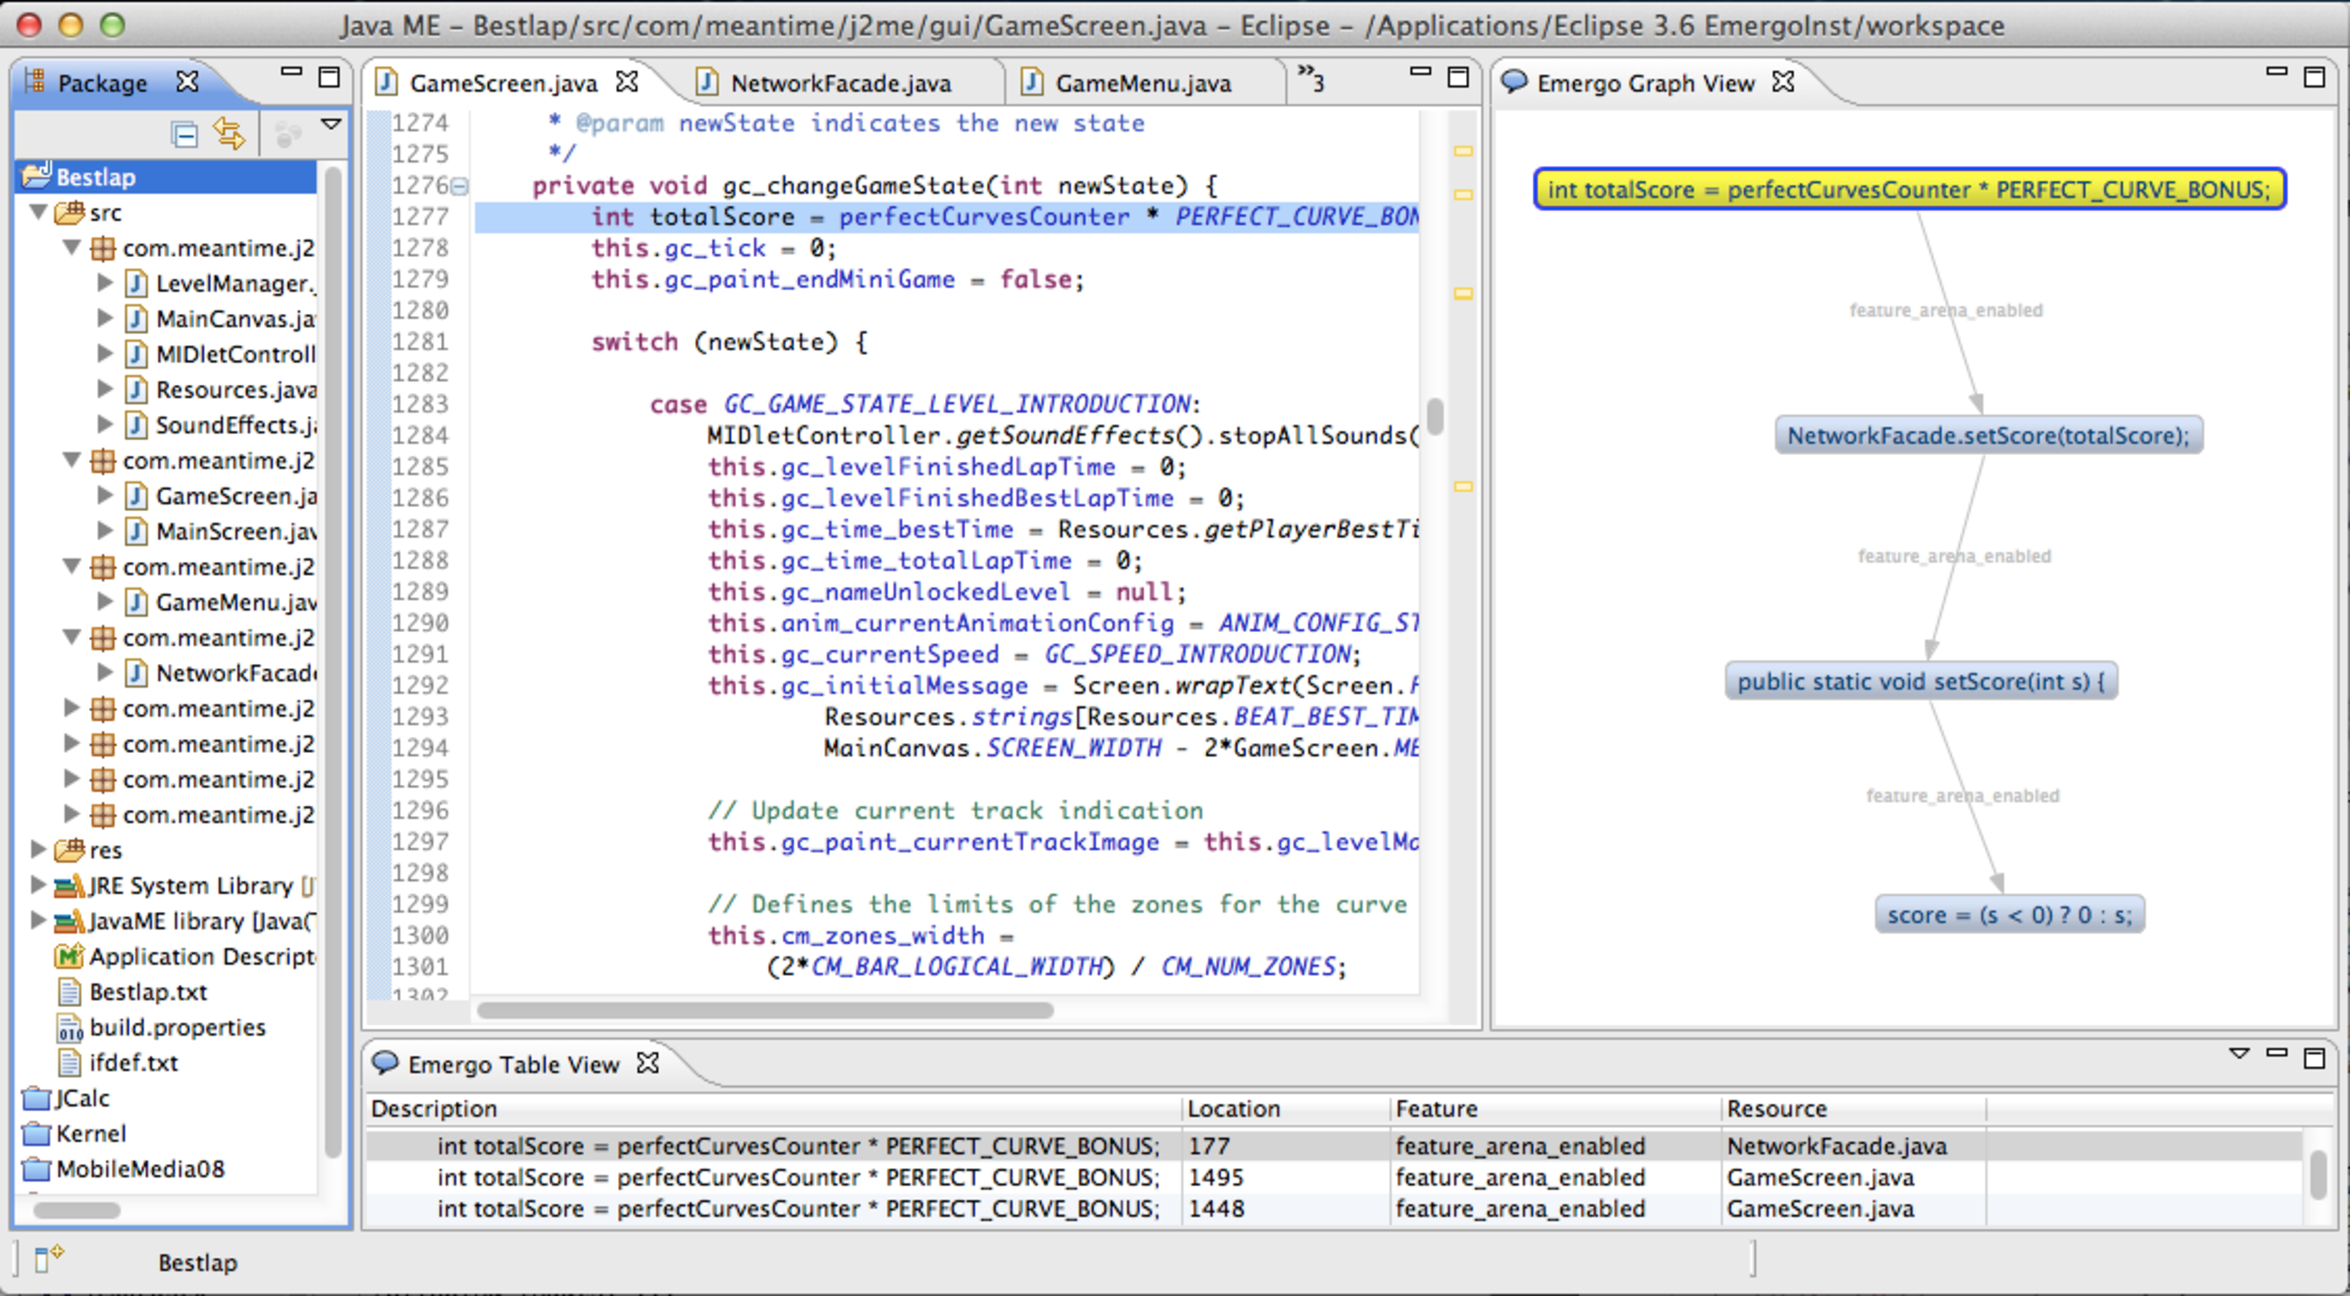
\includegraphics[width=.9\textwidth]{images/Emergo.pdf}
\caption{Emergent interface for Scenario 1 using Emergo.}
\label{fig:emergo}
\end{figure*}

Emergo can also help on preventing developers from analyzing unnecessary features and their associated code, which is important to decrease code change effort. In particular, we believe that Emergo can help on making the idea of virtual separation of concerns realistic. Thus, we can hide features and rely on Emergo to only open the ones we really need to. For instance, consider \textit{Scenario 2} (Section~\ref{sec:breaks}). Emergo would focus on \textit{CHOWN} and \textit{UTIMES}. So, we could keep \textit{SLINK} hidden, since it is not related to the current task.

Currently, our implementation has some limitations. To compute dependencies, we rely only on data-flow information, so we only compute data dependencies. Also, developers can only select maintenance points that range from simple variable assignments to code blocks that do not span to another method.

%containing assignments, method calls, and variable (local or class attributes) and method declarations. To compute interfaces for declarations, we also rely on AST-based analyses.

\subsection{Underlying Analysis}

The current implementation of Emergo computes interfaces based on data using \textit{interprocedural} and \textit{intraprocedural} feature-sensitive \textit{reaching-definition analysis}. So, from the maintenance points, we consider the reached program statements and their associated feature expressions to form our emergent interfaces. The feature-sensitive approach is capable of analyzing all configurations of a product line without having to generate all of them explicitly. This increases performance~\cite{brabrand-dfa4spl-aosd12, bodden-ifds4spl-pldi13}, which is important for interactive tools like ours that need to provide quick responses to developers requests. To perform the feature-sensitive analysis, we annotate the control-flow graph with feature information, lift the lattice to contain a mapping of sets of configurations to lattice values, and lift the transfer functions to figure out whether or not apply the ordinary function. The lifted function lazily splits the sets of configurations in two disjoint parts, depending on the feature expression annotated with the statement being analyzed: a set for which the function should be applied; and a set for which it should not~\cite{brabrand-dfa4spl-taosd12}.

%The current implementation of Emergo computes interfaces based on data using \textit{interprocedural} and \textit{intraprocedural} feature-sensitive reaching definition analysis. We also rely on AST-based analyses.

%\textbf{TODO explain in one or two paragraphs what kind of analysis is performed. move technical content from the previous section here.}

%\reviewer{Rev2: With regards to the technique of expressing and computing emergent interfaces, it is unclear what the input to the technique is. Is it a specific variable? A variable at a particular point in the code? An entire code block? A code block that spans more than one method? I would like to see much more clarity on the inputs to the mehod than provided by:}

%\reviewer{Figure 4 also made me question what the inputs and outputs are. How is the impacted feature shown? What is the feature in this example?}

%\idea{Maybe we should consider a complete screen shot of Emergo, instead of only considering the table view. We can do it since now we have some extra pages: 10 (icse) x 14 (oopsla).}

%\begin{figure}[htp]
%\centering
%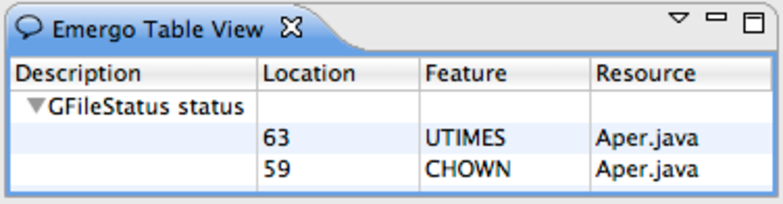
\includegraphics[width=0.45\textwidth]{images/Emergo-Table-View.pdf}
%\caption{Emergo view illustrating the impacted features. Lines 63 and 59 contain uses of \texttt{status}.}
%\label{fig:emergo-table-view}
%\end{figure}

%\reviewer{Rev1: That said, section III felt too short, especially if you have extended the tool. Some words on that and how it works would help.}

%\chk{from the description it is not clear how emergent interfaces are computed. you just say dataflow analysis, but that's probably littel help. you might want to describe at least in a few words when Emergo reports something, and how the analysis figures that out. possibly you might need to show a dataflow graph for one of the examples.}